\documentclass[../report.tex]{subfiles}

\usepackage{listings}
\usepackage{color}

\definecolor{dkgreen}{rgb}{0,0.6,0}
\definecolor{gray}{rgb}{0.5,0.5,0.5}
\definecolor{mauve}{rgb}{0.58,0,0.82}

\lstset{frame=tb,
  language=Sql,
  aboveskip=3mm,
  belowskip=3mm,
  showstringspaces=false,
  columns=flexible,
  basicstyle={\small\ttfamily},
  numbers=none,
  numberstyle=\tiny\color{gray},
  keywordstyle=\color{blue},
  commentstyle=\color{dkgreen},
  stringstyle=\color{mauve},
  breaklines=true,
  breakatwhitespace=true
  tabsize=3
}

\begin{document}
When designing the data model there were several considerations to make. Our design goals for the data model were as follows
\begin{itemize}
\item Make a generic data model that can suit both the ArtShare and the SMU Client.
\item Make the model as extensible as possible. By this we mean that we can add a new property to e.g. a \textit{Media item} without having to change the data model. This facilitates more iterative development.
\item We wanted our data model to be in the highest normal form possible to avoid redundancy in regards to data space and corruption
\end{itemize} 


%Firstly it was important to design a data model which was generic enough to accommodate the demands of the SMU team. Secondly it was important to design a data model which was in as high a normal form as possible in order to reduce redundant data and the possibility of creating corrupt data. Lastly we wanted to make the datamodel as extendible to new features as possible.  


%(WHY DID WE MAKE THE UPLOADER/OWNER OF A MEDIA ITEM A RELATION?!? NOW IT IS POSSIBLE FOR A MEDIA ITEM TO HAVE MORE THAN ONE UPLOADER/OWNER)


Looking at the requirements for \textit{The System} we identified two major entities, namely the \textit{User} and \textit{Media item}. Additionally we realised that we needed an entity representing a \textit{Client} in order for the \textit{ShareIt Back End} to be able to differentiate which \textit{Media Item}s belonged to which \textit{Client}. \\

\begin{figure}[H]
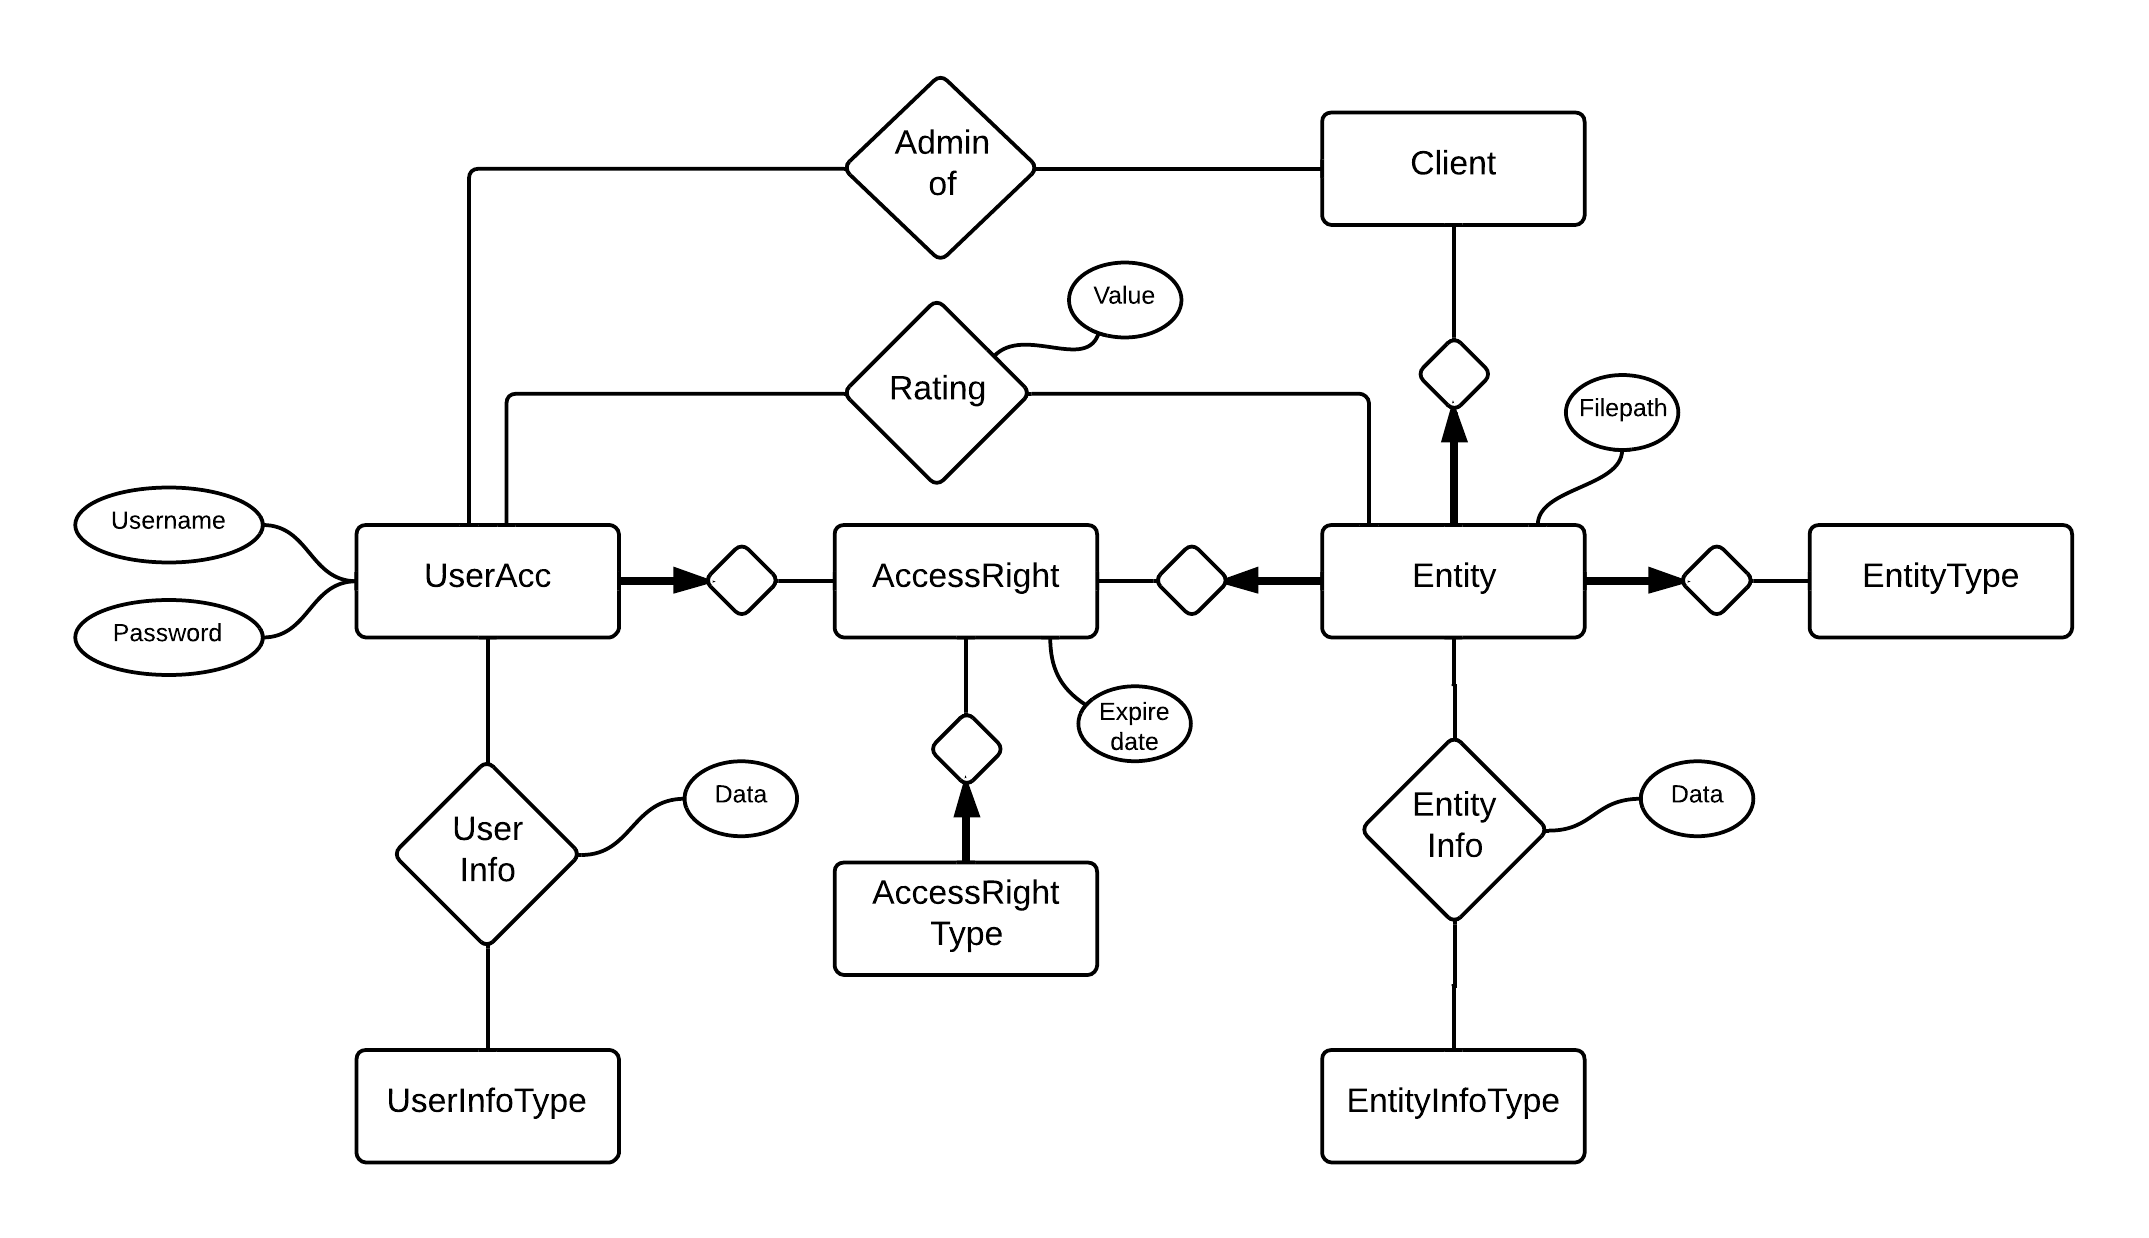
\includegraphics[width=\linewidth]{img/ER.png}
\caption{ER diagram of the data model}
\label{fig:use case diagram}
\end{figure}

In order to make the data model flexible and extensible we chose to only make the \textit{User} and \textit{Media item} carry required information while all other information, like title, artist, director, email etc., is made relational. This means that the \textit{Media item} is stored in three tables: Entity, EntityInfo and EntityInfotype (The SQL definition of \textit{Media Item} is shown fig \ref{datamodel}).

This both facilitates that clients can have different needs to which information is stored on a \textit{User} or \textit{Media item}, but also makes it easier to add more information types iteratively.\\

\begin{figure}[H]
\begin{lstlisting}
CREATE TABLE EntityInfoType(
	Id Int IDENTITY Primary Key,
	Name varchar(256) NOT NULL,
);

CREATE TABLE Entity(
	Id Int IDENTITY Primary Key,
	FilePath varchar(256) NOT NULL,
	ClientId Int NOT NULL REFERENCES Client(Id) ON DELETE CASCADE,
	TypeId Int REFERENCES EntityType(Id)
);

CREATE TABLE EntityInfo(
	Data varchar(max),
	EntityId Int NOT NULL REFERENCES Entity(Id) ON DELETE CASCADE,
	EntityInfoTypeId Int NOT NULL REFERENCES EntityInfoType(Id) ON DELETE CASCADE,
	Id INT IDENTITY Primary Key
);
\end{lstlisting}
\caption{Snippet of Entity (\textit{Media item}) SQL definition}
\label{datamodel}
\end{figure}

Another choice we made was to have an AccessRight relation between \textit{User}s and \textit{Media item}s. We made this choice to facilitate different access rights to a \textit{Media item} like Owner and Buyer.

Our data model is in 3NF (Third normal form). It is in 3NF and not BCNF (Boyce-Codd normal form) because we have IDs on all entities. An ID for e.g. \textbf{EntityInfo} (See figure \ref{datamodel} for table definition) is not needed as it could have been a weak entity. We have chosen to give it an ID either way because it was easier in regards to implementation of a generic Data Access Layer.

The full data model SQL definition can be found in appendix

(Move to appendix)

\begin{lstlisting}
CREATE TABLE Client(
	Id Int IDENTITY Primary Key,
	Name varchar(256) NOT NULL,
	Token varchar(256) NOT NULL
);

CREATE TABLE EntityInfoType(
	Id Int IDENTITY Primary Key,
	Name varchar(256) NOT NULL,
);

CREATE TABLE EntityType(
	Id Int IDENTITY Primary Key,
	Type varchar(256) NOT NULL UNIQUE
);

CREATE TABLE Entity(
	Id Int IDENTITY Primary Key,
	FilePath varchar(256) NOT NULL,
	ClientId Int NOT NULL REFERENCES Client(Id) ON DELETE CASCADE,
	TypeId Int REFERENCES EntityType(Id)
);

CREATE TABLE EntityInfo(
	Data varchar(max),
	EntityId Int NOT NULL REFERENCES Entity(Id) ON DELETE CASCADE,
	EntityInfoTypeId Int NOT NULL REFERENCES EntityInfoType(Id) ON DELETE CASCADE,
	Id INT IDENTITY Primary Key
);

CREATE TABLE UserAcc(
	Id INT IDENTITY Primary Key,
	Username varchar(20) NOT NULL UNIQUE,
	Password varchar(50) NOT NULL
);

CREATE TABLE UserInfoType(
	Id INT IDENTITY Primary Key,
	Type varchar(256) NOT NULL UNIQUE
);

CREATE TABLE UserInfo(
	Id Int IDENTITY Primary Key,
	Data varchar(max),
	UserId Int NOT NULL REFERENCES UserAcc(Id) ON DELETE CASCADE,
	UserInfoType Int NOT NULL REFERENCES UserInfoType(Id) ON DELETE CASCADE
);

CREATE TABLE AccessRightType(
	Id Int IDENTITY Primary Key,
	Name varchar(256) NOT NULL UNIQUE
);

CREATE TABLE AccessRight(
	Id Int IDENTITY Primary Key,
	Expiration datetime,
	EntityId Int NOT NULL REFERENCES Entity(Id) ON DELETE CASCADE,
	UserId Int NOT NULL REFERENCES UserAcc(Id) ON DELETE CASCADE,
	AccessRightTypeId INT NOT NULL REFERENCES AccessRightType(Id) ON DELETE CASCADE,
);

CREATE TABLE ClientAdmin(
	Id Int IDENTITY Primary Key,
	ClientId Int NOT NULL REFERENCES Client(Id) ON DELETE CASCADE,
	UserId Int NOT NULL REFERENCES UserAcc(Id) ON DELETE CASCADE	
);

CREATE TABLE Rating(
	Id int IDENTITY Primary Key,
	Value int NOT NULL,
	UserId Int NOT NULL REFERENCES UserAcc(Id) ON DELETE CASCADE,
	EntityId Int NOT NULL REFERENCES Entity(Id) ON DELETE CASCADE,
);
\end{lstlisting}




\end{document}